\documentclass{article}
\usepackage{amsmath,amsthm,amssymb}
\usepackage{mathtext}
\usepackage[T2A]{fontenc}
\usepackage[utf8]{inputenc}
\usepackage[english]{babel}
\usepackage{graphicx}
\usepackage{hyperref}


\title{Capsule Based Aspect Extraction}
\author{Kirill Krasikov}
\date{May 2020}



\begin{document}
\maketitle
\begin{abstract}
    In the world of data science, more and more data is required to train models. Getting labeled datasets is a very expensive and lengthy process. In this regard, in the problems of thematic modeling, aspect extraction models from unplaced text is gaining popularity. These models allow, with minimal effort to annotate aspects, to structure the text into a set of topics or intentions. In this paper, a comparison is made of a SotA model based on attention and a custom model in which the attention mechanism is replaced by a capsule network with dynamic routings. 
    Codes for paper: \url{https://github.com/KirillKrasikov/TopicModelingWithCapsNet}.
\end{abstract}



\section{Introduction}
Aspect extraction is an important and challenging task in aspect-based sentiment analysis. For example, in the sentence "The beef was tender and melted in my mouth", the aspect term is "beef". Two sub-tasks are performed in aspects extraction: (1) extracting all aspects terms(e.g., "beef") from a review corpus, (2) clustering aspect terms with similar meaning into categories where each category represents a single aspect(e.g., cluster "beef", "pork", "pasta", and "tomato" into one aspect food) \cite{He2018ABAE}. in 2017 year, Unsupervised Aspect Extraction \cite{He2018ABAE} have become the dominant unsupervised approach for aspect extraction. In that work neural word embeddings map words with the same context to nearby points in the embedding space \cite{Mikolov2013W2V}. Then attention mechanism \cite{Bahdanau2015NMT} filter the word embeddings within a sentence and filtered words use to construct aspect embeddings. The training process for aspect embeddings is analogous to autoencoders, where dimension reduction use to extract the common factors among embedded sentences and reconstruct each sentence through a linear combination of aspect embeddings. The attention mechanism deemphasizes words that are not part of any aspects, allowing the model to focus on aspect words. That model call \textit{Attention-based Aspect Extraction} (ABAE). In the same year "Google brain" suggested approach called \textit{Dynamic Routing Between Capsules} \cite{Hinton2017DRBC}. A capsule is a group of neurons whose activity vector represents the instantiation parameters of a specific type of entity such as an object or an object part. The length of the activity vector use to represent the probability that the entity exists and its orientation use to represent the instantiation parameters. Active capsules at one level make predictions, via transformation matrices, for the instantiation parameters of higher-level capsules. When multiple predictions agree, a higher level capsule becomes active. To best performance use iterative routing-by-agreement mechanism: A lower-level capsule prefers to send its output to higher level capsules whose activity vectors have a big scalar product with the prediction coming from the lower-level capsule \cite{Hinton2017DRBC}. In this work i implement ABAE model using pytorch, then change attention mechanism to capsule network and evaluate this models on Citysearch corpus used by previous works \cite{Ganu2009BeyondTheStars} \cite{Brody2010UAS} \cite{Zhao2010JMA} \cite{He2018ABAE}.


\section{Related Work}
\label{sec:related}
The problem of aspect extraction has been well studied in the past decade. Initially, methods were mainly based on manually defined rules. \cite{HuLiu2004} proposed to extract different product features through finding frequent nouns and noun phrases. They also extracted opinion terms by finding the synonyms and antonyms of opinion seed words through WordNet. Following this, a number of methods have been proposed based on freequent item mining and dependency information to extract product aspects \cite{Zhuang2006} \cite{Somasundarn2009} \cite{Qiu2011}. These models heavily depend on predefined rules which work well only when the aspect terms are restricted to a small group of nouns. Supervised learning approaches generally model aspect extraction as a standard sequence labeling problem. \cite{Jin2009} \cite{Li2010} proposed to use hidden Markov models(HMM) and conditional random fields(CRF) respectively with a set of manually-extracted features. More recently, different neural models \cite{Yin2016} \cite{Wang2016} were proposed to automatically learn features for CRF-based aspect extraction. Rule-based models are usually not refined enough to categorize the extracted aspect terms. On the other hand, supervised learning requires large amounts of labeled data for training purposes.

Unsupervised approaches, especially topic models, have been proposed subsequently to avoid reliance on labeled data. Generally, the outputs of those models are word distributions or rankings for each aspect. Aspects are naturally obtained without separately performing extraction and categorization. Most existing works \cite{Brody2010UAS} \cite{Zhao2010JMA} \cite{Mukherjee2012} \cite{Chen2014} are based on variants and extensions of LDA \cite{Blei2003}. Recently, \cite{Wang2015} relies on a substantial amount of prior knowledge such as part-of-speech(POS) tagging and sentiment lexicons. A biterm topic models (BTM) that generates co-occurring word pairs was proposed in \cite{Yan2013}.

Attention models \cite{Mnih2014} have recently gained popularity in training neural networks and have been applied to various natural language processing tasks, including machine translation \cite{Bahdanau2015NMT}, sentence summarization \cite{Rush2015}, sentiment classification \cite{Chen2016} and question answering \cite{Herman2015}. Rather than using all available inforamtion, attention mechanism aims to focus on the most pertinent information for a task. \cite{He2018ABAE} apply attention to an unsupervised neural model and demonstrate its effectiveness for aspect extraction.

\cite{Zhao2018} explore capsule networks with dynamic routing process \cite{Hinton2017DRBC} for supervised text classification. In this work i apply capsule network with dynamic routing to unsupervised neural model and evaluate experimental results with ABAE and others aspect extraction models. 

\section{Model Description}

The ultimate goal of Capsule Based Aspect Extraction (CBAE) is to learn a set of aspect embeddings, where each aspect can be interpreted by looking at the nearest words (representative words) in the embedding space. Each word $w$ in vocabulary with a feature vector $e_w \in \R^d$ \cite{He2018ABAE}. Word embeddings use to map words that often co-occur in a context to points that are close by in the embedding space \cite{Mikolov2013W2V}. The feature vectors associated with the words correspond to the rows of a word embedding matrix $E \in R^{Vd}$, where $V$ is the vocabulary size. Model try to learn embeddings of aspects, where aspects share the same embedding space with words. This requires an aspect embedding matrix $T \in R^{Vd}$, where $K$ - the number of aspects ($K$ much smaller than $V$). The aspect embeddings are use to approximate the aspect words in the vocabulary, where aspects words are filtered through an capsule network with dynamic routing\footnote{This is a key difference from ABAE \cite{He2018ABAE} , in which the mechanism of attention is used to filtering words to aspects.}.
Each input sample to CBAE is a list of indexes for words in a review sentence. First, the model filter away non-aspects words by down-weighting them using an capsule network and construct a sentence embedding $z_s$ from weighted word embeddings. Then, the model try to reconstruct the sentence embedding as a linear combination of aspect embedding from $T$. This process of dimension reduction and reconstruction, where CBAE aims to transform sentence embeddings of the filtered sentences ($z_s$) into their reconstruction ($r_s$) with the least possible amount of distortion, preserves most of the information of the aspect words in the K embedded aspects. This process is described in detail in \cite{He2018ABAE}.

\subsection{Sentence Embedding and Capsule Network with dynamic routing}

Capsule network, depicted in Fig.~\ref{fig:capsule} get sentence embedding vector to input. It consists of four layers: n-gram convolutional layer, primary capsule layer, secondary capsule layer and fully connected capsule layer. 

\begin{figure}[!tbh]
    \centering
    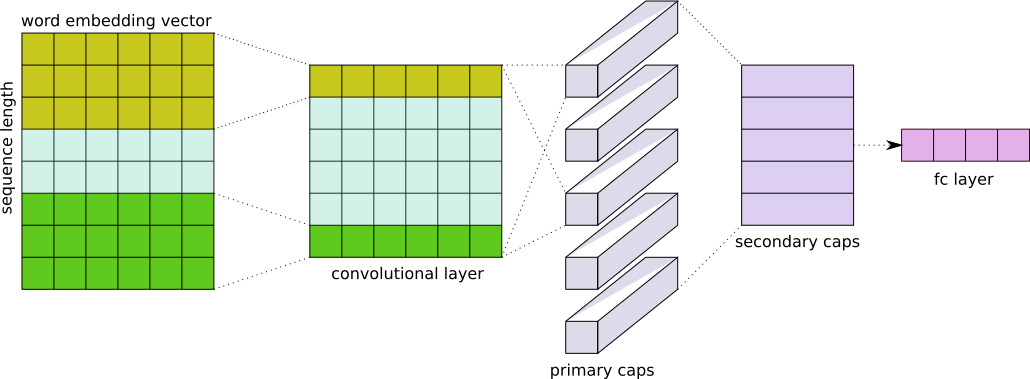
\includegraphics[width=1\linewidth]{rect10315.png}
    \caption{The Architecture of capsule network for aspect extraction (CBAE encoder part)}
    \label{fig:capsule}
\end{figure}

N-gram convolutional layer is a standard convolutional layer which extracts n-gram features at different positions of a sentence through various convolutional filters\cite{Zhao2018} and activated by ELU function. Primary capsule layer is the first capsule layer in which the capsules replace the scalar-output feature detectors of CNNs with vector-output capsules to preserve the instantiated parameters sush as the local order of words and semantic representation of words. Capsule network tries to address the representational limitation and exponential inefficiencies of convolutions with transformation matrices \cite{Hinton2017DRBC}. It allows the networks to automatically learn child-parent relationships constituting viewpoint invariant knowledge that automatically generalizes to novel viewpoints. Dynamic routing need to construct a non-linear map in an iterative manner ensuring that the output of each capsule get sent to an appropriate parent in the subsequent layer. For each potential parent, the capsule network can increase or decrease the connection strength by dynamic routing, which is more effective than the primitive routing strategies such as max-pooling in CNN that essentially detects whether a feature is present in any position of the text, but loses spatial information about the feature. Secondary capsule layer multiply transformation matrices to learn child-parent relationships followed by routing agreement to produce parent capsules in the above. Then the capsules from secondary capsule layer flattened into fully connected final capsule then activate by tanh function and normalize by softmax.


\section{Dataset}
The model have been evaluated on \textbf{Citysearch corpus}. This is restaurant review corpus widely used by previous works \cite{Ganu2009BeyondTheStars} \cite{Brody2010UAS} \cite{Zhao2010JMA}, which contains over 50,000 restaurant reviews from Citysearch New York. \cite{Ganu2009BeyondTheStars} provided a subset of 3,400 sentences from the corpus with manually labeled aspects. These annotated sentences are used for evaluation of aspect identification. There are six manually defined aspect labels: \textit{food}, \textit{staff}, \textit{ambience}, \textit{price}, \textit{anecdotes} and \textit{miscellaneous}. Corpus prerocessing and word2vect model described in \cite{He2018ABAE}.


\section{Experiments}

\subsection{Metrics}
The model was evaluated by precision, recall and F1 scores. Сlasses of aspects were put down manually.

\subsection{Experiment Setup}
For the CBAE and ABAE implementation i repeat parametrs from \cite{He2018ABAE}.  Initialize the word embedding matrix E with word vectors trained by word2vec with negative sampling on each dataset, setting the embedding size to 200, windows size to 10 and negative sample size to 5. The aspect embedding matrix initialized with the centroids of clusters results resulting from running $k$-means on word embeddings. Other parameters are initialized randomly. During the training process word embedding matrix $E$ was fixed, other parameters optimized using Adam with learning rate 1e-3 for 10 epoch and batch size of 50. The number of negative samples was set to 20. Following \cite{Brody2010UAS}, \cite{Zhao2010JMA}, \cite{He2018ABAE} the number of aspect for the corpus was set to 14. In CBAE like an ABAE, representative  words of an aspect can be found by looking at its nearest words in the embedding space using cosine as the similarity metric.

\subsection{Baselines}
To validate the performance of CBAE, the model compare with next baselines:

1) \textbf{LocLDA} \cite{Brody2010UAS}: This method uses a standard implementation of LDA.

2) \textbf{$k$-means} \cite{He2018ABAE}: Aspect matrix T with k-means centroids of the word embeddings.

3) \textbf{SAS} \cite{Mukherjee2012}: Hybrid topic model that jointly discovers both aspects and aspect-specific opinions.

4) \textbf{BTM} \cite{Yan2013}: Bitermic topic model that is specially designed for short texts such as texts from social media and review sites. The major advantage of BTM over conventional LDA models is that it alleviates the problem of data sparsity in short documents by directly modeling the generation of unordered word-pair co-occurrences (biterms) over the corpus.

5) \textbf{ABAE} \cite{He2018ABAE}: Attention based aspect extraction scores from original papper.

6) \textbf{ABAEr}: ABAE replication on pytorch without ortho regularization.


\section{Results}
Tab.~\ref{tab:aspects} presents all 14 aspects inferred by CBAE. The inferrent aspects are more finegrained then standard labels.

\begin{table}[tbh!]
\begin{center}
\begin{tabular}[t]{l|l|l}
\hline
 Inferred Aspects & Representative Words & Gold Aspects \\
\hline
todo & todo & todo  \\
\hline
\end{tabular}
\caption{List of inferred aspects for restaurant reviews (left), with top representative words for each inferred aspect (middle), and the corresponding gold-standard aspect labels (right). Inferred aspect labels (left) were assigned manually.}
\label{tab:aspects}
\end{center}
\end{table}

Evaluation criterion of sentence-level-aspects identification is to judge how well the predictions match the true labels, measured by precision, recall and $F_1$ scores. The results are shown in Tab .~\ref{tab:eval}

\begin{table}[tbh!]
\begin{center}
\begin{tabular}[t]{l|l|l|l|l}
\hline
 Aspect & Method & Precision & Recall & $F_1$ \\
\hline
todo & todo & todo & todo & todo  \\
\hline
\end{tabular}
\caption{Aspect identification results on the restaurant domain. The results of LocLDA and MELDA are taken from \cite{Zhao2010JMA}; the results of SAS and SERBM are taken from \cite{Wang2015}; the results of k-means and ABAE are taken from \cite{He2018ABAE}}.
\label{tab:eval}
\end{center}
\end{table}


\section{Conclusion}
TODO

\bibliographystyle{apalike}
\bibliography{lit}
\end{document}
